% =========================================================================== %

\begin{frame}[t,plain]
\titlepage
\end{frame}

% =========================================================================== %

\begin{frame}[fragile]{Variadic Functions -- Variable Zahl von Argumenten}
%
\begin{columns}[T]
\column{.45\linewidth}
\begin{itemize}
\item Vgl. \texttt{printf}: Beliebige Zahl von Ausgabe-Parametern
\item Umsetzung über \emph{variadic functions}
\item Prototyp/Funktions-Signatur enthält \texttt{...} als letztes Argument
\item Handling über Funktionen und Makros aus \texttt{stdarg.h}
\item Intern: Übergabe eines \mintinline{c}{void *} für Daten und eines \mintinline{c}{int *} für Datenmenge
\item \texttt{va\_list} -- Datentyp, enthält beide Pointer
\end{itemize}
%
\column{.55\linewidth}
\begin{codebox}[Syntax: Funktions-Signatur]
\begin{minted}[fontsize=\scriptsize]{c}
return_type funcName(fixed_arguments, ...);
\end{minted}
\end{codebox}
%
\begin{itemize}
\item \texttt{va\_start(list, count)} -- Makro. Speichert Pointer von Typ \texttt{va\_list} in Variable \texttt{list}. Parameter \texttt{count} ist Zahl der Werte in der Liste.
\item \texttt{va\_arg(list, type)}  -- Makro, liest den nächsten Wert aus Liste \texttt{list} von Typ \texttt{va\_list}; Wert selbst ist vom Typ \texttt{type}.
\item \texttt{va\_end(list)} -- Makro, gibt Speicher für Liste \texttt{list} wieder frei.
\end{itemize}
\end{columns}
%
\end{frame}

% =========================================================================== %

\begin{frame}[fragile]
%
\begin{minipage}{.49\linewidth}
\begin{codebox}[Beispiel: Standardabweichung ...]
\begin{minted}[fontsize=\scriptsize, linenos]{c}
#include <stdio.h>
#include <stdarg.h>
#include <math.h>
 
double stddev(int count, ...) {
   double sum = 0, sum_sq = 0, num;
   
   va_list args;   
   va_start(args, count);
   
   for (int i = 0; i < count; ++i) {
      num = va_arg(args, double);
      sum    += num;
      sum_sq += num * num;
   }
   va_end(args);
   
   return sqrt(sum_sq / count - 
      (sum / count) * (sum / count));
}
\end{minted}
\end{codebox}
\end{minipage}
%
\begin{minipage}{.49\linewidth}
\begin{codebox}[... Fortsetzung (von \href{https://en.cppreference.com/w/c/variadic/va_arg}{cppreference})]
\begin{minted}[fontsize=\scriptsize, linenos, firstnumber=last]{c}
int main(void) 
{
   printf(
      "Std. deviation of list: %f\n", 
      stddev(
         4, 
         25.0, 27.3, 26.9, 25.7
      )
   );
}
\end{minted}
\end{codebox}
%
\vspace{-4pt}
\begin{hintbox}[Definition: Standardabweichung]
\footnotesize Statistisches Maß für Streuung einer Messreihe $(x_i)_{i=1,\ldots,n}$ um Mittelwert 
$\overline{x}$.
\[
\sigma = \sqrt{
	\frac
		{\sum^{n}_{i=1}(x_i - \overline{x})^2}
		{n}
}
\]
\end{hintbox}
\end{minipage}
%
\end{frame}

% =========================================================================== %

\begin{frame}{GTK+}
%
\begin{itemize}
\item GIMP Toolkit
	\begin{itemize}
	\item Entstanden als Routinen-Sammlung für Grafikprogramm GIMP
	\item Freie Software unter \emph{LGPL}
	\end{itemize}
\item Multi-Plattform: Code funktioniert unter Linux genauso wie unter Windows oder Mac
\item Verschiedene Versionen im Umlauf
	\begin{itemize}
	\item GTK+ v1 -- 1998 bis 2002 -- ca  93.000 lines of code
	\item GTK+ v2 -- bis 2004 -- ca 558.000 lines of code -- heute verbreitetste Version
	\item GTK+ v3 -- Weiterentwicklung bis heute -- 
		Mehr Flexibilität, noch nicht auf allen Systemen Teil der Standard-Installation
	\item \url{https://people.redhat.com/mclasen/Usenix04/notes/x29.html}
	\end{itemize}
\item Kurs orientiert sich an online-Tutorial:\\
	\url{https://developer.gnome.org/gtk-tutorial/stable/}
\item Versionen nicht kompatibel, Grundsätzliche Logik aber dieselbe
\end{itemize}

%
\end{frame}

% =========================================================================== %

\begin{frame}[fragile]{GTK+ 2.0 -- Eine GUI-API}
%
\begin{columns}[T]
\column{.5\linewidth}
\begin{itemize}
\item GUI: Graphical User Interface
\item API: Application Programming Interface
\item[$\Rightarrow$] Große Routinen-Sammlung
\item Verweist auf ca 100 \emph{Header} und vorkompilierte Programmbibliotheken
\item Einbinden geschieht automatisch über mehrere Macros in Code und Compileraufruf
\item \texttt{pkg-config}: Linux-Tool: Gibt Informationen über Komponenten eines \emph{packages} (Software-Paket) aus.
\end{itemize}
%
\column{.5\linewidth}
\begin{codebox}[Compiler-Kommando]
\begin{minted}[fontsize=\scriptsize]{text}
gcc 
   myCodefile1.c myCodefile2.c ...
   -lm -lglut -lGL
   -std=c99 -Wall 
   `pkg-config --cflags --libs gtk+-2.0`
   -o myExecutable
\end{minted}
\end{codebox}
%
\begin{itemize}
\item Information hier nur der Vollständigkeit halber -- jeder Programmierer automatisiert das
\item[$\Rightarrow$] Script \texttt{crg}
\end{itemize}
\end{columns}
%
\end{frame}

% =========================================================================== %

\begin{frame}{GTK -- Grundlegendes Herangehen}
%
\begin{columns}[T]
\column{.5\linewidth}
\begin{itemize}
%\item Einbinden der Bibliotheken mit \mintinline{c}{#include <gtk/gtk.h>}
\item Bibliotheken laden und initialiseren
\item \emph{Widgets} (Objekte  wie z.\,B. Fenster, Buttons, ...) definieren: Größe, Position,
	Beschriftung, ...
\item \emph{Signale} und \emph{Events}
	\begin{itemize}
	\item Ereignis, auf das reagiert werden kann. 
	\item Beispiele: Mausklick, Tastaturdruck, ...
	\item Benutzerdefinierte Signale möglich
	\item Beispiel: Spiel; Computergegner hat Zug beendet $\Rightarrow$ Controllbuttons wieder frei geben
	\end{itemize}
\end{itemize}
%
\column{.5\linewidth}
\begin{itemize}
\item \emph{Callback-Functions}
	\begin{itemize}
	\item Code, der bei \emph{Signal} ausgelöst wird
	\item Function Pointers
	\end{itemize}
\item Zuordnung: Signal $\rightarrow$ Callback Function
\item Hierarchische Gliederung der Widgets
	\begin{itemize}
	\item Button ist \enquote{im} Fenster
	\item[$\Rightarrow$] Effekte auf Fenster betreffen auch Button
	\item Sprechweise \emph{Parent} und \emph{Child}
	\item Mehrere Schachtelungs-Ebenen (z.\,B. Gruppen von Buttons)
	\end{itemize}
\end{itemize}
\end{columns}
%
\end{frame}

% =========================================================================== %

\begin{frame}{Kontrollübergabe an GTK}
%
\begin{itemize}
\item Nachdem alle Widgets vorbereitet wurden: GTK übernimmt Kontrolle über Programmfluss
\item Intern: Endlos-Schleife, reagiert auf Signale und verteilt diese weiter
\item Endlos-Schleife ruft unsere Callback-Funktionen auf.
\item Am Ende der Callback-Funktionen: Wieder Rückkehr in \texttt{gtk\_main}
\item[$\Rightarrow$] keine eigenen Endlosschleifen möglich.
\item Manche Signale gehen an das GTK-System selbst
\item Beispiel: \texttt{gtk\_main\_quit} -- Beende das \emph{gesamte} Programm.
\end{itemize}
%
\end{frame}

% =========================================================================== %

\begin{frame}{Zentrales Objekt: \texttt{GtkWidget}}
%
\begin{itemize}
\item Objekt: Fenster, Button, Textbox, ..., aber 
\item Alle Objekte werden als \texttt{GtkWidget *} angelegt
\item Zusammengesetztes Objekt, ähnlich \texttt{FILE *}
\item Funktionen aus dem GTK-Katalog nehmen Variablen dieses Typs an oder geben solche Pointer zurück
\item Automatische Freigabe bei Programmende -- Internes Management durch GTK-Funktionen
\item Sammlung von Routinen und GTK-Objekten:\\
	\url{https://developer.gnome.org/gtk2/stable/ch02.html}
\end{itemize}
%
\end{frame}

% =========================================================================== %

\begin{frame}[fragile]{Objekte Anlegen}
%
\begin{columns}[T]
\column{.5\linewidth}
\begin{itemize}
\item Verschiedene Funktionen für verschiedene Objekte
\item Sehr ähnliche Grundstruktur\\
	\texttt{gtk\_[widget-name]\_new}
\item Abwandlungen davon existieren: Direkte Zuweisung von Start-Werten
\item Parameter \texttt{GTK\_WINDOW\_TOPLEVEL}: Erstelle \enquote{normales} Fenster; Variante für Popups
\item Details: Siehe Referenz
\end{itemize}
%
\column{.5\linewidth}
\begin{codebox}[GTK-Widgets anlegen -- zwei Beispiele]
\begin{minted}[fontsize=\scriptsize]{c}
GtkWidget *window = gtk_window_new (
   GTK_WINDOW_TOPLEVEL);

GtkWidget *button = 
   gtk_button_new_with_label (
      "Hello World"
   );
\end{minted}
\end{codebox}
%
\begin{itemize}
\item \footnotesize \url{https://developer.gnome.org/gtk2/stable/GtkWindow.html}
\item \url{https://developer.gnome.org/gtk2/stable/GtkButton.html}
\end{itemize}
\end{columns}
%
\end{frame}

% =========================================================================== %

\begin{frame}[fragile]{Signale Verknüpfen}
%
\begin{columns}[T]
\column{.45\linewidth}
\begin{itemize}
\item Mit Signal wird übermittelt: Auslöser, Signal-Art, Optionale Informationen
\item Zur Verknüpfung also nötig: Diese drei, plus: Callback-Funktion
\item Erledigt von Funktion \texttt{g\_signal\_connect}
\item viele neue Datentypen -- meist aliase für primitive Typen
\item Signatur der Callback-Funktion muss zum Signal passen
\end{itemize}
%
\column{.55\linewidth}
\begin{codebox}[g\_signal\_connect -- Funktionssignatur]
\begin{minted}[fontsize=\scriptsize]{c}
gulong g_signal_connect(
   gpointer      *object,
   const gchar   *name,
   GCallback     func,
   gpointer      func_data );

void callback_func( 
   GtkWidget *widget,
   /* other signal arguments */
   gpointer   callback_data );
\end{minted}
\end{codebox}
%
\begin{itemize}
\item Link zum Abschnitt im Tutorial: \\
	\footnotesize\url{https://developer.gnome.org/gtk-tutorial/stable/x159.html}
\end{itemize}
\end{columns}
%
\end{frame}

% =========================================================================== %

\begin{frame}[fragile]
%
\tcbset{width=.495\linewidth, on line, height=7.7cm}
%
\begin{codebox}[Beispiel: GTK: Hello World ...]
\begin{minted}[fontsize=\scriptsize, linenos]{c}
#include <gtk/gtk.h>

// callback funcs delete_event, 
//   destroy and hello

int main(int argc, char **argv) {
   gtk_init (&argc, &argv);
   
   GtkWidget *window, *button;
    
   window = gtk_window_new 
      (GTK_WINDOW_TOPLEVEL);
   g_signal_connect (
      window, "delete-event",
      G_CALLBACK (delete_event), NULL);
   g_signal_connect (
      window, "destroy",
      G_CALLBACK (destroy), NULL);   
   gtk_container_set_border_width (
      GTK_CONTAINER (window), 10);
\end{minted}
\end{codebox}
%
\begin{codebox}[Beispiel: ...Fortsetzung]
\begin{minted}[fontsize=\scriptsize, linenos, firstnumber=last]{c}
   button = gtk_button_new_with_label (
      "Hello World");
   g_signal_connect (
      button, "clicked",
      G_CALLBACK (hello), NULL);
   g_signal_connect_swapped (
      button, "clicked",
      G_CALLBACK (gtk_widget_destroy),
      window);
    
   gtk_container_add (
      GTK_CONTAINER (window), button);
    
   gtk_widget_show (button);
   gtk_widget_show (window);
    
   gtk_main ();
    
   return 0;
}
\end{minted}
\end{codebox}
%
\end{frame}

% =========================================================================== %

\begin{frame}[fragile]{gtk\_hello\_world.c im Detail -- Signale des Fensters}
%
\begin{minted}[fontsize=\footnotesize]{c}
g_signal_connect (window, "delete-event", G_CALLBACK(delete_event), NULL);
g_signal_connect (window, "destroy",      G_CALLBACK(destroy)     , NULL);
\end{minted}
%
\begin{itemize}
\item Handling von Programmende: \texttt{destroy}-Signal und \texttt{delete-event}
	\begin{itemize}
	\item \texttt{delete-event}: \texttt{[ALT] + [F4]}, Schließen-Button, oder ähnliches
	\item \texttt{destroy}: Löschen eines einzelnen Widgets -- auch für Buttons, etc.
	\end{itemize}
\item \enquote{Emitter} des Signals: Hauptfenster \texttt{window}
\item Signal- bzw. Event-Namen als Strings (\mintinline{c}{char *})
\item Handling durch Callbacks (\texttt{delete\_event}, \texttt{destroy}) -- werden später besprochen
\item Type-Casting und Prüfung der Signatur durch Makro \texttt{G\_CALLBACK}
\item Letzter Parameter: Pointer auf evtl. notwendige zusätzliche Daten -- 
	\mintinline{c}{NULL} für \enquote{keine Daten}
\end{itemize}
%
\end{frame}

% =========================================================================== %

\begin{frame}{gtk\_hello\_world.c im Detail -- Fenstereigenschaften steuern}
%
\mint{c}{gtk_container_set_border_width (GTK_CONTAINER (window), 10);}
%
\begin{minipage}{.6\linewidth}
\begin{itemize}
\item Konzept \emph{Container}
	\begin{itemize}
	\item Graphische Umgebung, in der Widgets angezeigt werden können.
	\item Mehrere Widgets können in einen Container \enquote{gepackt} werden.
	\item An sich eigenständiges \texttt{GtkWidget}, aber auch automatisch in manchen Widgets
		implementiert -- z.\,B. im \texttt{window}.
	\item Makro \texttt{GTK\_CONTAINER}: Spreche den Container des Widgets an
	\end{itemize}
\item Ähnlich: Titelleiste, Fenstergröße, ... ändern
\end{itemize}
\end{minipage}
%
\begin{minipage}{.39\linewidth}
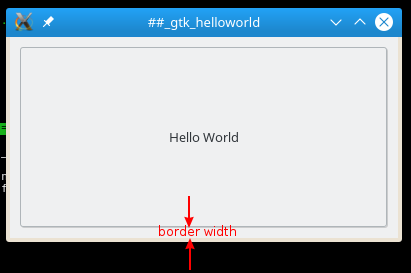
\includegraphics[width=\linewidth]{./gfx/gtkHelloWorld}
\end{minipage}
%
\end{frame}

% =========================================================================== %

\begin{frame}[fragile]{gtk\_hello\_world.c im Detail -- Signale des Buttons}
%
\begin{minted}[fontsize=\footnotesize]{c}
g_signal_connect         (button, "clicked", G_CALLBACK (hello), NULL);
g_signal_connect_swapped (button, "clicked", G_CALLBACK (gtk_widget_destroy), window);
\end{minted}
%
\begin{itemize}
\item Mehrere Handler mit selbem Signal und selbem Emitter verknüpfbar -- werden hierarchisch abgearbeitet
\item Erste Verknüpfung damit klar -- Aufruf von Function \texttt{hello} bei Klick auf Button
\item \texttt{g\_signal\_connect\_swapped}
	\begin{itemize}
	\item Selber Effekt -- Aufruf einer Funktion bei Klick
	\item Andere Signatur der aufgerufenen Funktion
	\item Hier: Aufruf einer gtk-Funktion, daher swapped notwendig
	\item Sendet \texttt{destroy}-Signal an Fenster
	\end{itemize}
\end{itemize}
%
\end{frame}

% =========================================================================== %

\begin{frame}[fragile]{gtk\_hello\_world.c im Detail -- Packen, Sichtbarkeit, Start!}
%
\begin{minted}[fontsize=\footnotesize]{c}
gtk_container_add (GTK_CONTAINER (window), button);
gtk_widget_show (button);
gtk_widget_show (window);
gtk_main ();
\end{minted}
%
\begin{itemize}
\item \texttt{gtk\_container\_add}
	\begin{itemize}
	\item In Container (1. Parameter) das Widget (2. Parameter) packen
	\item Damit auch Parent-Child-Hierarchie bestimmt
	\item Container von Window: Kann nur 1 Child aufnehmen
	\item Child kann aber selbst auch wieder Container sein
	\item Verschiedene Container-Arten, alle fassen mehrere Widgets
	\end{itemize}
\item \texttt{gtk\_widget\_show}
	\begin{itemize}
	\item Sichtbarkeits-Flag setzen
	\item Gegenbefehl: \texttt{gtk\_widget\_hide}
	\end{itemize}
\item \texttt{gtk\_main} -- Kontrolle an GTK abgeben.
\end{itemize}
%
\end{frame}

% =========================================================================== %

\begin{frame}[fragile]
%
\begin{minipage}{.5\linewidth}
\begin{codebox}[Callback-Funcs in gtk\_helloworld ...]
\begin{minted}[fontsize=\scriptsize, linenos]{c}
static void hello(
   GtkWidget *widget,
   gpointer   data
) {
   g_print ("Hello World\n");
}

static gboolean delete_event( 
   GtkWidget *widget,
   GdkEvent  *event,
   gpointer   data
) {
   g_print ("delete event occurred\n");
   return TRUE;
}
\end{minted}
\end{codebox}
\end{minipage}
%
\begin{minipage}{.49\linewidth}
\begin{codebox}[... Fortsetzung]
\begin{minted}[fontsize=\scriptsize, linenos, firstnumber=last]{c}
static void destroy( 
   GtkWidget *widget,
   gpointer   data 
) {
   gtk_main_quit ();
}
\end{minted}
\end{codebox}
%
\begin{itemize}
\item \texttt{hello} -- Gibt \texttt{Hello World} auf Konsole aus
\item \texttt{delete\_event} -- gibt Text auf Konsole aus, verhindert Programm-Ende
\item \texttt{destroy} -- beendet das Programm
\end{itemize}
\end{minipage}
%
\end{frame}

% =========================================================================== %

\begin{frame}[fragile]{Callback-Funktionen im Detail: \texttt{hello}}
%
\begin{minipage}{.5\linewidth}
%
\begin{itemize}
\item Schlüsselwort \mintinline{c}{static} bei Functions
	\begin{itemize}
	\item Sichtbarkeit nur in der aktuellen Translationseinheit
	\item Compiler-Aufruf erlaubt mehrere Code-Files. $\Rightarrow$ Translationseinheit\\
		Beispiel: \texttt{gcc soure1.c source2.c -o output}
	\item \mintinline{c}{#include} -- Teil derselben Einheit
	\end{itemize}		
\item \texttt{g\_print}
	\begin{itemize}
	\item Textausgabe über benutzerdefinierten \emph{Handler}
	\item Standard: direkte Weitergabe an \texttt{printf}
	\item Beliebige andere Functions können hier ansetzen
	\item Nützlich z.\,B. für Ausgabe auf Fenster
	\end{itemize}
\end{itemize}
\end{minipage}
%
\begin{minipage}{.49\linewidth}
\begin{codebox}[Function \texttt{hello}]
\begin{minted}[fontsize=\scriptsize, linenos]{c}
static void hello(
   GtkWidget *widget,
   gpointer   data
) {
   g_print ("Hello World\n");
}
\end{minted}
\end{codebox}
%
\begin{itemize}
\item Parameter 1 \texttt{widget}: auslösendes Widget
\item[$\Rightarrow$] Mehrere Widgets, selbe Funktion
\item Parameter 2 \texttt{data} -- beliebige Daten
\item Parameter müssen entgegen genommen werden, auch wenn nicht verarbeitet
\end{itemize}
\end{minipage}
%
\end{frame}

% =========================================================================== %

\begin{frame}[fragile]{Callback-Funktionen im Detail: \texttt{delete\_event} und \texttt{destroy}}
%
\begin{minipage}{.5\linewidth}
\begin{itemize}
\item Unterschiedliche Signaturen
	\begin{itemize}
	\item \texttt{delete\_event} reagiert auf ein \emph{event}
	\item Rückgabetyp \texttt{gboolean} -- \texttt{TRUE}/\texttt{FALSE}
	\item Zusätzlicher Parameter \texttt{event} -- Details zum Event
	\item Beispiel: Event \texttt{mousemove}: Koordinaten
	\end{itemize}
\item \texttt{delete\_event}
	\begin{itemize}
	\item Textausgabe und Rückgabe \texttt{TRUE}\\
		Event-Handling abgeschlossen \\
		$\Rightarrow$ Programm nicht beendet
	\item \texttt{FALSE}: Weiterleitung $\rightarrow$ Standard-Handler
	\end{itemize}
\item \texttt{destroy}
	\begin{itemize}
	\item Beendet Progamm über gtk-Funktion
	\end{itemize}
\end{itemize}
\end{minipage}
%
\begin{minipage}{.49\linewidth}
\begin{codebox}[\texttt{delete\_event} und \texttt{destroy}]
\begin{minted}[fontsize=\scriptsize, linenos]{c}
static gboolean delete_event( 
   GtkWidget *widget,
   GdkEvent  *event,
   gpointer   data
) {
   g_print ("delete event occurred\n");
   return TRUE;
}

static void destroy( 
   GtkWidget *widget,
   gpointer   data 
) {
   gtk_main_quit ();
}
\end{minted}
\end{codebox}
\end{minipage}
%
\end{frame}